\documentclass{article}

\usepackage[english]{babel}
\usepackage[utf8x]{inputenc}
\usepackage{amsmath}
\usepackage{graphicx}
\usepackage[colorinlistoftodos]{todonotes}

\title{Evaluate}
\author{Jordan Matelsky}

\begin{document}
\maketitle

\section{Introduction}

\section{Improvement Strategies}

\subsection{Baseline}
The baseline provided had an accuracy rate of 0.449312, which means that it functioned slightly better than chance (which would have chosen uniformly from ${-1, 0, 1}$ with probability $0.33...$. This strategy uses a sort of word-union calculation, where the only metric for calculating accuracy is the intersect of words that occur in a hypothesis and its reference sentence.

More formally, for reference sentence $r$ and hypothesis $h$:

$$A = \big| \{ w | w \in h, w \in r \} \big|$$

I provide several modifications in this assignment, as well as advantages and disadvantages for each.

\subsection{WordNet Synonym Lookup}
This strategy is a very slight modification of the previous implementation, wherein a word is counted as a $+1$ if it exists in both sentences ($h$ and $r$), and a word $w$ from a hypothesis is counted as a $+p$ (for some $p \in 0..1$) if $synonym(w) \in r$.

$synonym(w)$ is defined using Princeton's WordNet system, accessed via RESTful API endpoint through \texttt{thesaurus.altervista.org}.

\subsubsection{Advantages}
This protocol supposedly casts a wider net to find more sentences that may have simply mistranslated a word but still retain the `gist' of a sentence — such as in cases where ``ball'' is replaced with ``sphere'', etc.

\subsubsection{Disadvantages}
Because this system relies on an internet connection and the WordNet API, it is very slow to execute (in my trials, it took nearly nine wallclock minutes to run 100 sentences). Moreover, accuracy is diminished, as it appears that this `dragnet' approach considers too many sentences to be correct.

\subsubsection{Results}
\textit{See Table 1.}  From the above information, it is likely that the strategy used here is useful for tie-breaking, but is not a viable strategy as a standalone device.

\subsection{METEOR}
For this implementation, I use the METEOR formula as described in the homework prompt \texttt{mt-class.org/jhu/hw3.html}, namely:

$$\displaystyle \ell(h,e) = \frac{P(h,e) \cdot R(h,e)}{(1-\alpha)R(h,e) + \alpha P(h,e)}$$

The only deviation I implemented handles the case of $P(h,e) = R(h,e) = 0$, wherein my implementation (intuitively, at least to me) returns $0$, indicating zero correlation.

\subsubsection{Advantages}
This system has clear advantages over the baseline strategy — namely, it maximizes the cases in which two sentences are similar enough to be considered `close' while still minimizing those cases due to chance. It is essentially a sliding-scale version of the baseline implementation. However, the pure METEOR implementation can be improved upon, as I will explore below.

\subsubsection{Disadvantages}
METEOR is naïve and still fails on cases where sentences use synonyms. It also fails to accommodate sentence structure in any way, so the sentences \textit{the the the the the} and \textit{the the} are weighted equally.

\subsubsection{Results}
This implementation functions notably better than the baseline implementation, reaching approximately $50\%$ accuracy on the provided dataset. For further evaluation statistics, see \textit{Figure \ref{fig:meteoralpha}}.

\subsection{Quorum}
After performing the above implementations, I decided to try to improve the accuracy at the expense of performance by running multiple algorithms and having them reach `quorum'. To do this, I modified the \texttt{evaluate} function to take an array of tuples for \texttt{eval\_fns}, in the form:

$$(function, weight)$$

Using only METEOR and $n=20$, I arrived at an accuracy of $0.5$. Using the Quorum implementation mixing METEOR at 75\% weight and WORDNET at 25\% weight, I arrived at an accuracy of 0.55.

\subsubsection{Advantages}
On $n=20$, accuracy from METEOR alone (0.5) was improved by combining with WORDNET (combined, led to $A=0.55$).

\subsubsection{Disadvantages}
Naturally, the combined algorithm takes considerably longer to run, and if WORDNET is among the utilized algorithms, it performs far slower (as WORDNET requires HTTP calls).

To improve timing, I added a dynamic element that added words and their synonyms to a dictionary (local) as it encountered them over HTTP, so that subsequent calls ran faster. For timing figures, see \textit{Figure \ref{fig:dynamic}}.




%%%%%%%%%%%%%%%%%%%%%%%% Figures %%%%%%%%%%%%%%%%%%%%%%%%

\begin{table}[tbp]
\centering
\caption{WordNet Sentence Intersect Results}
\label{t1}
\begin{tabular}{llll}
Pred. y=-1          & y=0 & y=1 &    \\
True y=-1           & 19  & 7   & 18 \\
True y= 0           & 7   & 7   & 9  \\
True y= 1           & 19  & 2   & 12 \\
                    &     &     &    \\
A = 0.380000 &  (n=100)     &     &
\end{tabular}
\end{table}

\begin{table}[tbp]
\centering
\caption{METEOR}
\label{t2}
\begin{tabular}{llll}
Pred.               & y=-1 & y=0 & y=1  \\
True y=-1           & 6315 & 899 & 3748 \\
True y= 0           & 1722 & 487 & 1724 \\
True y= 1           & 3642 & 841 & 6190 \\
                    &      &     &      \\
A = 0.508135 & ($\alpha=0.75$)     &     &
\end{tabular}
\end{table}

\begin{figure}[ht]
\caption{A plot of $\alpha$ values ($x$) against accuracy ($y$).}
\label{fig:meteoralpha}
\centering
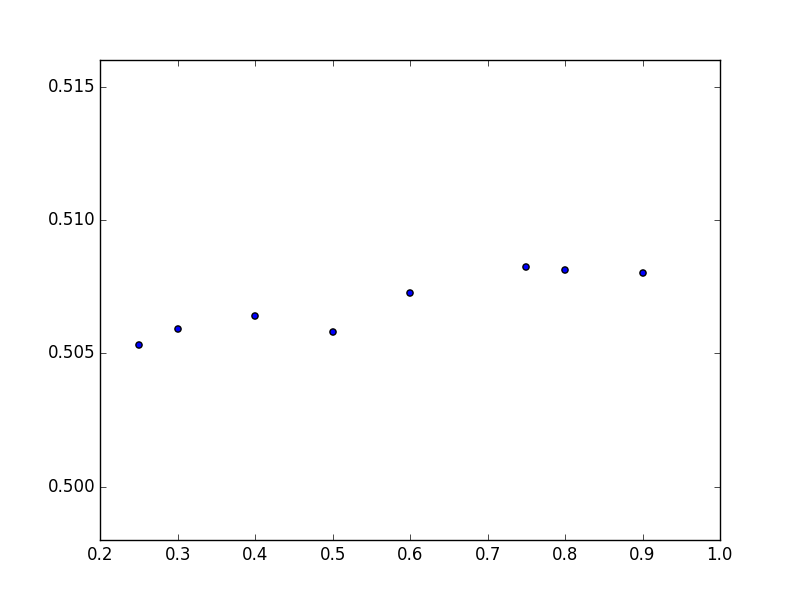
\includegraphics[width=0.5\textwidth]{figure_1}
\end{figure}

\begin{figure}[ht]
\caption{Naive speeds when running WORDNET (red) compared with dynamic version (blue), which saves the encountered words to a local dictionary for faster lookup.}
\label{fig:dynamic}
\centering
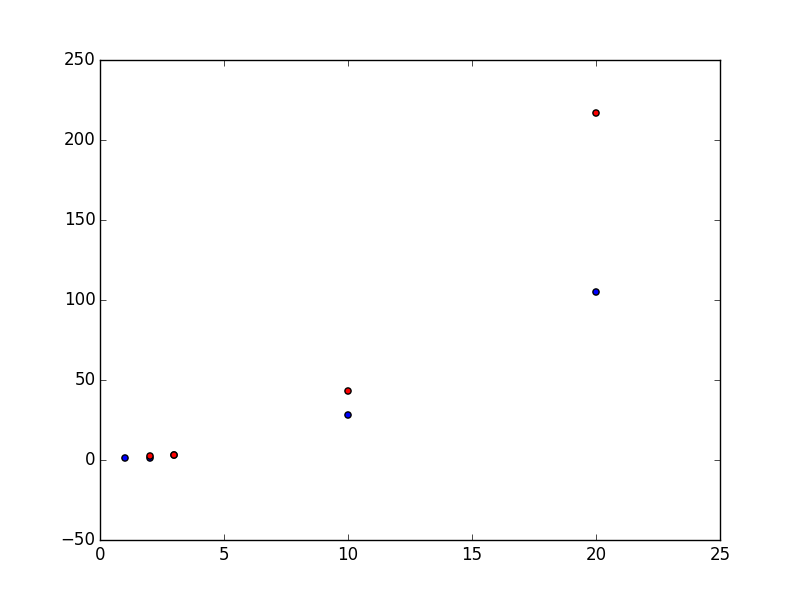
\includegraphics[width=0.5\textwidth]{figure_2}
\end{figure}

\end{document}
